\chapter{Testy nowej metody}

W tym rozdziale zostaną przedstawione testy i walidacja opracowanej metody, przedstawionej w Rozdziale \ref{NewMethod}. W pierwszej kolejności zaprezentowane zostanie porównanie z metodą wytrenowaną z wykorzystaniem paradygmatu end-to-end, a zatem explicite modelującą ocenę radiologa. Następnie metoda przedstawiona przez autora tej pracy zostanie porównana z wynikami prac algorytmu oceniającego proces gojenia się ścięgna Achillesa z wykorzystaniem danych z Ultrasonografii. Finalnie, ostateczny test dotyczyć będzie zestawienia wyników z oceny biomechanicznej z zaproponowanym w poprzednim rozdziale podejściem.

Zarówno metoda oparta o paradygmat end-to-end jak i o dane Ultrasonograficzne są wynikiem prac, w których autor tej rozprawy był współautorem i nadzorował grupę studentów opracowujących finalne rozwiązania oraz tworzył plan badań. W przypadku oceny biomechanicznej prace nad metodą zrealizowane zostały w całości przez mgr Magdalenę Syrek z Carolina Medical Center w Warszawie, zatem wartością dodaną tej rozprawy jest przedstawione w dalszej części porównanie.   

\section{Porównanie z metodą opartą o paradygmat end-to-end}

W tej sekcji opracowana metoda zostanie porównana z metodą opartą o paradygmat end-to-end, modelującą explicite ocenę radiologa. Do tego zadania zostały wykorzystane trzy architektury sieci konwolucyjnych opisane w Rozdziale \ref{CNNs} tj. AlexNet, GoogLeNet (Inceptionv3) i ResNet z 50 warstwami konwolucyjnymi (ResNet-50). Wszystkie trzy architektury zostały zmodyfikowane poprzez zastąpienie końcowej warstwy klasyfikacyjnej warstwą regresji z pojedynczym wyjściem i funkcją kosztu zdefiniowaną jako średni błąd kwadratowy. W skutek tego podejścia algorytm szkolony jest, aby minimalizować błąd pomiędzy predykcją sieci neuronowej, a wartościami parametrów z wzorca odniesienia. 

Do szkolenia się sieci wykorzystano pełny zestaw treningowy tj. 44 pacjentów ograniczony do trzech protokołów wybranych w toku eksperymentów przedstawionych w podsekcji \ref{seq:protocol_selection}: T2 $^\ast$ GRE, T2 $^\ast$ GRE TE\_MIN i PD. Tym razem nie zdecydowano się na zawężenie zbioru danych tylko do jednej sekwencji RM z uwagi na próbę maksymalizację liczebności zbioru. Do szkolenia zastosowano metodę kroswalidacji z podziałem na 4 segmenty. Dla każdego z parametrów z wzorca odniesienia wyszkolono osobną sieć. Wyliczono matryki MAE, MAX-AE i Corr stosowane również w poprzednim rozdziale. Wyniki zestawiono w Tab. \ref{tab:end-to-endTrain}.
%\vspace{-8px}
\begin{table}[ht]
%\vspace{-px}
\scriptsize
\setlength{\tabcolsep}{1pt}
\centering
\caption{Wyniki szkolenia się sieci w paradygmacie end-to-end z wykorzystaniem zbioru treningowego.}
\label{tab:end-to-endTrain}
\begin{tabular}{lc||c|c|c|c|c|c}
	%\hline
	&& \textbf{SCT} & \textbf{TT} & \textbf{STE} & \textbf{TE} & \textbf{TU} & \textbf{TisE}\\ \hline
	\textbf{AlexNet$_{e}$} & MAE & \textbf{1.04}$\pm$0.33 & \textbf{0.82}$\pm$0.27 & \textbf{0.95}$\pm$0.48 & \textbf{0.88}$\pm$0.38 & \textbf{1.03}$\pm$0.36 & \textbf{0.78}$\pm$0.26  \\
	&MAX-AE & 1.91 & 1.67 & 2.39 & 2.20 & 1.90 & 1.35\\ 
	&Corr & 0.82 & 0.72 & 0.13 & 0.70 & 0.50 & 0.83 \\ \hline
	\textbf{Inceptionv3$_{e}$} & MAE & \textbf{0.88}$\pm$0.32 & \textbf{0.75}$\pm$0.22 & \textbf{0.82}$\pm$0.33 & \textbf{0.78}$\pm$0.20 & \textbf{0.91}$\pm$0.34 & \textbf{0.67}$\pm$0.23 \\
	&MAX-AE & 1.57 & 1.44 & 1.93 & 1.17 & 1.85 & 1.11 \\ 
	&Corr & 0.85 & 0.72 & 0.05 & 0.72 & 0.52 & 0.84 \\ \hline
	\textbf{ResNet-50$_{e}$} & MAE & \textbf{0.64}$\pm$0.21 & \textbf{0.98}$\pm$0.28 & \textbf{0.83}$\pm$0.37 & \textbf{0.89}$\pm$0.22 & \textbf{1.06}$\pm$0.41 & \textbf{1.10}$\pm$0.34  \\
	&MAX-AE & 1.21 & 1.79 & 1.94 & 1.43 & 2.42 & 2.36\\
	&Corr & 0.06 & 0.21 & 0.00 & 0.11 & 0.14 & 0.11\\
	
	
\end{tabular}
%\vspace{-0.5cm}
\end{table}

Otrzymane wartości MAE znajdują się w zakresie 0.64 to 1.10 (w skali wzorca odniesienia 0--7). Dla najlepszego modelu pod względem średniej MAE tj. Inceptionv3, średni dystans między predykcją i wzorcem wyniósł $<0.92$. Najlepiej estymowanymi parametrami były TisE -- 0.67, TT -- 0.75 i TE -- 0.78. Najgorsze rezultaty natomiast otrzymano dla TU -- 0.91, który to parametr silnie zależy od informacji widocznej w płaszczyxnie strzałkowej.

W kolejnej tabeli (Tab. \ref{tab:end-to-end_testset}) przedstawiono zestawienie automatycznej oceny dla zbioru pacjentów testowych, realizowanego przed najlepszy model szkolony w paradygmacie end-to-end (IncepionV3) i proponowaną przez autora tej pracy metodą (SVR).  

\begin{table*}[t]
	\caption{Test set results for the tendon healing progression.}
	\scriptsize
	\begin{center}
		\begin{tabular}{lc||c|c|c|c|c|c}
			\textbf{Model} & & \textbf{SCT} & \textbf{TT} & \textbf{STE} & \textbf{TE} & \textbf{TU} & \textbf{TisE}\\ 
			
\hline
%			AlexNet$_{e}$ &MAE & 1.33$\pm$0.64 & 0.87$\pm$0.11 & $1.38\pm{0.75}$ & 1.16$\pm{0.24}$ & 1.10$\pm{0.27}$& 0.90$\pm{0.19}$ \\
%			& MAX-AE & 2.28 & 1.02 & 2.48 & 1.34 & 1.39 & 1.12 \\ 
%			& Corr & 0.79 & 0.54 & 0.0 & 0.50 & 0.16 & 0.66 \\ \hline
			Inceptionv3$_{e}$ & MAE & 1.12$\pm{0.74}$ & 0.80$\pm{0.24}$ & 1.40$\pm{0.52}$ & \textbf{0.89}$\pm{0.31}$ & 1.08$\pm{0.26}$ & \textbf{0.69}$\pm{0.07}$ \\
			& MAX-AE & 2.14 & \textbf{1.01} & 2.13 & \textbf{1.18} & 1.44 & \textbf{0.78} \\
			& Corr & \textbf{0.82} & \textbf{0.77} & 0.05 & 0.59 & 0.02 & \textbf{0.77} \\ \hline
%			ResNet-50$_{e}$  & MAE & \textbf{0.62}$\pm{0.35}$ & 0.94$\pm0.39$ & 0.94$\pm0.29$ & 1.12$\pm{0.12}$ & 1.08$\pm{0.14}$ & 0.97$\pm{0.43}$ \\
%			& MAX-AE & \textbf{0.93} & 1.52 & \textbf{1.27} & 1.28 & \textbf{1.21} & 1.45 \\
%			& Corr & 0.20 & 0.55 & 0.11 & 0.19 & 0.12 & 0.37\\
%			\hline \hline
			SVR & MAE & $1.05\pm0.12$ & $0.56\pm0.06$ & $0.75\pm0.08$ & $0.91\pm0.10$ & $0.91\pm0.09$ & $0.94\pm0.10$\\
			& MAX-AE & 2.62 & 1.82 & 1.92 & 2.54 & 2.01 & 2.38 \\
			& Corr   & 0.85 & 0.85 & 0.31 & 0.72 & 0.65 & 0.80 
		\end{tabular}
	\end{center}
	\label{tab:end-to-end_testset}
\end{table*}

Metoda SVR osiąga wyższe rezultaty Corr w każdym z parametrów i niższe MAE dla 4 z 6 parametrów. Natomiast tylko w jednym z parametrów (tj. STE) charakteryzuje się niższym MAX-AE. 

Można zatem wnioskować, że cechy wykorzystywane w metodzie SVR do oceny procesu gojenia się skuteczniej dywersyfikują kolejne fazy procesu i pozwalają na ocenę trendu z lepszą dokładnością niż metoda oparta o paradygmat end-to-end. 2 z 6 parametrów, w których pod względem MAE sieć InceptionV3 okazała się lepsza tj. TE i TisE dotyczą obrzęków, zatem elementów ocenianych pod kątem pola powierzchni i kształtu. Fakt ten należy interpretować, iż tego rodzaju informacja dominuje w ekstrahowanych przez jądra splotu obrazach, co z kolei implikuje gorsze wyniki w pozostałych parametrach ocenianych na podstawie wzorców tworzonych przez struktury ścięgniste. Wynik MAX-AE nie jest zaskakujący, ponieważ z uwagi na naturę treningu (explicite modelowanie wzorca odniesienia) maksymalne błędy będą minimalizowane. Trudność w interpretacji polega na fakcie, że maksymalne błędy mogą być wynikiem błędu algorytmu jak również pojedynczymi omyłkami doświadczonego radiologa, który z uwagi np. na zmęczenie bądź inne dystrakcje zaburzające percepcję, popełnił błąd w ocenie.  

W tym kontekście należy również podkreślić zasadnicze różnice między dwoma przedstawionymi metodami. Do rozwoju metody end-to-end niezbędna jest pełna informacja od radiologa tj. ocena 6 parametrów w kolejnych krokach czasowych. Średnio jest to około 1 godziny na pacjenta. Proponowana przez autora metoda może być dalej rozwijana przy wykorzystaniu danych oznaczonych jako chory, zdrowy oraz znacząco mniejszego zbioru pacjentów z oznaczonym pełnym wzorcem odniesienia, który posłużyłby do sporadycznych ulepszeń etapu meta-regresji. Co prawda metoda wymaga również informacji o ROI, jednakże jest to czas około 10 minut na pacjenta, dla radiologa wykorzystującego odpowiednie oprogramowanie np. Osirix [X] lub VisNow [X]. Ponadto segmentację ROI można stosunkowo łatwo zautomatyzować. Wstępne prace dr. Jędrzeja Nowosielskiego i dr. Piotra Regulskiego oraz autora tej pracy pokazują, że skuteczne w tym zakresie mogą być sieci typu \textit{fully convolutiona neural networks}. Przykład działania takiej architektury (tj. U-Net [X]) można zaobserwować na Rys. \ref{fig:segmentacja}. 

\begin{figure}[h]
	\centering
	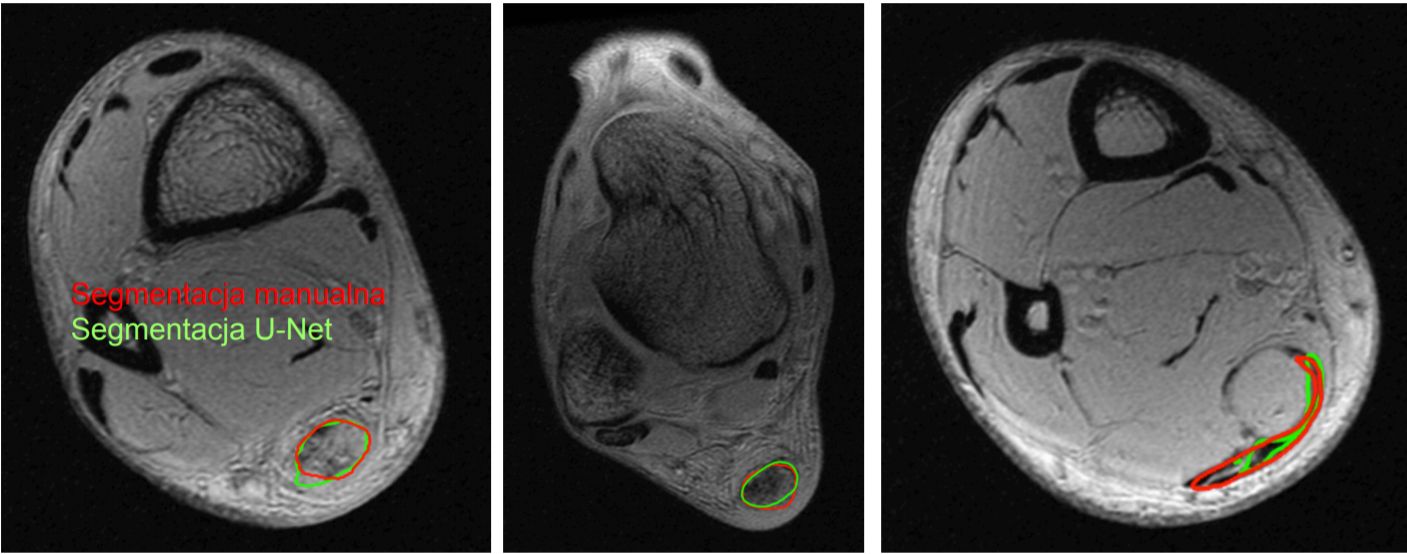
\includegraphics[width=1\textwidth]{figures/Segmentacja.png}
	\caption{Automatyczna segmantacja ROI z wykorzystaniem głębokich sieci neuronowych.}\label{fig:segmentacja}
\end{figure}

Kolorem czerwonym oznaczono obszar segmentacji manulanej, wykonanej przez eksperta radiologa. Kolorem zielonym efekt segmentacji automatycznej. Miara DICE dla otrzymanych obrazów wynosi około 0.75 i świadczy o wysokiej jakości segmentacji oraz o obiecującym kierunku tego rodzaju prac.

Ciekawym elementem rozwoju automatycznej oceny byłaby również fuzja obu metod tj. podmiana ekstraktora cech DL trenowana na binarnie oznaczonym zbiorze na ekstraktor uzyskanego modelu InceptionV3. Jednak z uwagi na omawiane problemy praktyczne z dalszym rozwojem tak utworzonej metody oraz brak obiecujących rezultatów w przeprowadzonych przez autora tej pracy badaniach wstępnych, taka propozycja nie została uwzględniona w prezentowanej rozprawie. 

\section{Porównanie z metodą opartą o dane z ultrasonografii}
\section{Porównanie z metodą opartą o badania biomechaniczne}


\chapter{Podsumowanie}
%- jeden radiolog więc ankieta ok
%- AlexNet uczy się bardziej generycznych cech niż ResNet, który zwraca uwagę na szczególy: https://www.researchgate.net/post/Can_AlexNet_be_a_better_feature_extractor_than_ResNet

%https://icmlviz.github.io/icmlviz2016/assets/papers/4.pdf